\section{Case Study}

We have used the Object Algebras framework in the implementation of a simple DSL for Questionnaires, called QL~\cite{GPCE}.
A questionnaire is rendered as an interactive form where, depending on user actions, new questions may appear, or values may be computed. 
QL programs consist of lists of labeled, typed questions.
Questions can be answerable, meaning the user has to enter some data, or computed.
In the latter case the question is defined by an expression.
A conditional if-then-else construct allows questions to visually appear only when a certain condition is true. 

To illustrate the utility of \name we have implemented a number of queries and transformations in the context of QL. The queries extract derived information from a QL program, such as the set of used variables, the data and control dependencies between questions and the type environment.
The transformations include two transformations of language extensions to the base language.
The first realizes a simple desugaring of ``unless(c){...}'' to ``if(not(c)){...}''.
The second desugaring statically unfolds a constant bound loop construct (``repeat (i){...}'') and renames variables accordingly.
Finally, we have implemented a simple rename variable operation, and a normalizer which flattens nested conditionals to sequences.  

Table~\ref{TBL:qlresults} shows the number of cases that had to be overridden to implement each particular operation. The top row shows the number of  constructs for each sort in QL (Exp, Stmt, and Form, respectively).
As can be seen, none of the operations required implementing all cases.
For this set of queries and transformations, almost no expression cases needed to be overridden, except the ``Var'' case in collect variables, rename variable and desugar ``repeat''\footnote{Note, however, that the dependency extraction queries reuse the collect variables query on expressions.}.
The cases required for desugaring include the case of the language extension, which is not counted in the total in the top row. 

\begin{table}[t]
  \centering
  \begin{tabular}{l|c|c|c}
    Operation            & Exp (18) & Stmt (5) & Form (1) \\\hline
    Collect variables    & 1              &                &               \\
    Data dependencies    &                & 3               & 1             \\
    Control dependencies &                & 4              & 1             \\
    Type environment     &                & 2              &               \\\hline
    Rename variable      & 1              & 2              &               \\
    Inline conditions    &                & 4              &               \\
    Desugar ``unless''   &                & 1              &               \\
    Desugar ``repeat''   & 1              & 3              &               \\
  \end{tabular}
  \caption{Number of overriden cases per query and transformation in
    the context of the QL implementation\label{TBL:qlresults}}
\end{table}


\subsection{Desugaring Language Extensions}



\subsection{\name performance vs Vanilla ASTs}


\begin{figure}
  \centering
  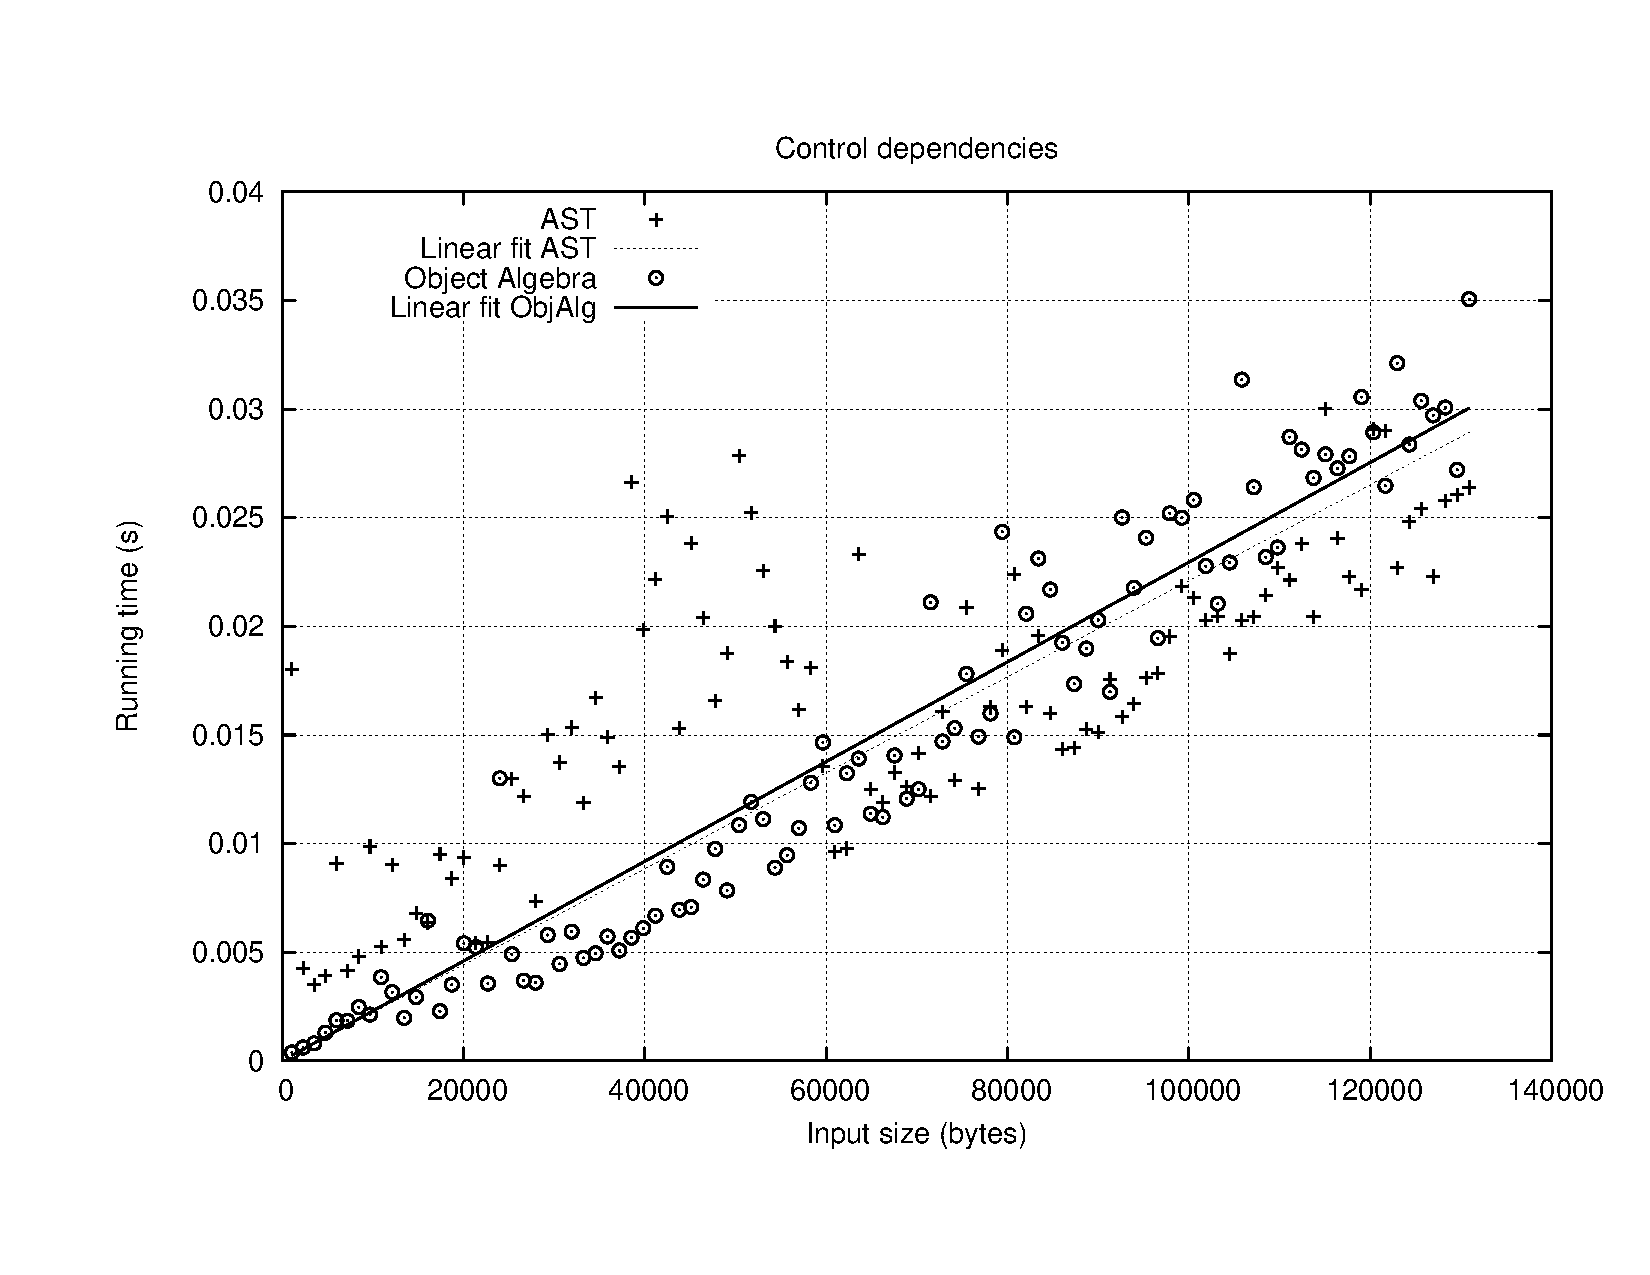
\includegraphics[width=0.8\textwidth]{plots/controldeps}
  \caption{Performance of control dependencies query implemented using normal ASTs vs using the \name framework\label{FIG:perfControlDeps}}
\end{figure}

